%%%%%%%%%%%%%%%%%%%%%%%%%%%%%%%%%%%%%%%%%
% Beamer Presentation - LaTeX Template
% Version 2.0 (March 8, 2022)
% Original Template: https://www.LaTeXTemplates.com
% Author: Vel (vel@latextemplates.com)
% License: CC BY-NC-SA 4.0

% Este modelo de apresentação foi 
% criado a partir do modelo de Giovanni Spadaro.
% Disponível em: https://github.com/Giovo17/presentation-template-unict-lm-data
%
% Adaptado por Lucas Amaral Taylor para criar uma versão especial 
% para os alunos de Matemática e Estatística da USP (IME-USP).
% Disponível em: https://github.com/lucasamtaylor01/IME-template
%%%%%%%%%%%%%%%%%%%%%%%%%%%%%%%%%%%%%%%%%

%----------------------------------------------------------------------------------------
% CLASSE DO DOCUMENTO E CONFIGURAÇÕES BÁSICAS
%----------------------------------------------------------------------------------------
\documentclass[
    12pt,               % Tamanho padrão da fonte
    % t,                % Alinhar verticalmente ao topo
    aspectratio=169,   % Definir proporção 16:9
]{beamer}
\graphicspath{{img/}}         % Define o diretório das imagens

%----------------------------------------------------------------------------------------
% PACOTES NECESSÁRIOS
%----------------------------------------------------------------------------------------
\usepackage{
    booktabs,     % Melhora a aparência das linhas em tabelas
    palatino,     % Define Palatino como fonte principal
    subcaption    % Suporte para subfiguras
}
\usepackage[default]{opensans}  % Define Open Sans como fonte secundária
%----------------------------------------------------------------------------------------
%	PACOTES E CONFIGURAÇÕES PARA CÓDIGO
%----------------------------------------------------------------------------------------
% Pacotes necessários para formatação de código
\usepackage[utf8]{inputenc}
\usepackage{listings}
\usepackage{xcolor}

% Cores para syntax highlighting (VSCode Light Theme)
\definecolor{vscBackground}{RGB}{255,255,255}    % Fundo branco
\definecolor{vscKeyword}{RGB}{175,0,219}         % Roxo para palavras-chave
\definecolor{vscString}{RGB}{163,21,21}          % Vermelho para strings
\definecolor{vscComment}{RGB}{0,128,0}           % Verde para comentários
\definecolor{vscFunction}{RGB}{121,94,38}        % Marrom para funções
\definecolor{vscNumber}{RGB}{9,134,88}           % Verde escuro para números
\definecolor{vscOperator}{RGB}{175,0,219}        % Roxo para operadores
\definecolor{vscText}{RGB}{0,0,0}                % Texto preto
\definecolor{vscLineNr}{RGB}{128,128,128}        % Cinza para números de linha

% Configuração geral do listings para UTF-8
\lstset{
    inputencoding=utf8,
    extendedchars=true,
    literate=%
        {á}{{\'a}}1 {é}{{\'e}}1 {í}{{\'i}}1 {ó}{{\'o}}1 {ú}{{\'u}}1
        {Á}{{\'A}}1 {É}{{\'E}}1 {Í}{{\'I}}1 {Ó}{{\'O}}1 {Ú}{{\'U}}1
        {à}{{\`a}}1 {è}{{\`e}}1 {ì}{{\`i}}1 {ò}{{\`o}}1 {ù}{{\`u}}1
        {À}{{\`A}}1 {È}{{\'E}}1 {Ì}{{\`I}}1 {Ò}{{\`O}}1 {Ù}{{\`U}}1
        {ã}{{\~a}}1 {ẽ}{{\~e}}1 {ĩ}{{\~i}}1 {õ}{{\~o}}1 {ũ}{{\~u}}1
        {Ã}{{\~A}}1 {Ẽ}{{\~E}}1 {Ĩ}{{\~I}}1 {Õ}{{\~O}}1 {Ũ}{{\~U}}1
        {â}{{\^a}}1 {ê}{{\^e}}1 {î}{{\^i}}1 {ô}{{\^o}}1 {û}{{\^u}}1
        {Â}{{\^A}}1 {Ê}{{\^E}}1 {Î}{{\^I}}1 {Ô}{{\^O}}1 {Û}{{\^U}}1
        {ç}{{\c c}}1 {Ç}{{\c C}}1
        {º}{{\textordmasculine}}1
        {ª}{{\textordfeminine}}1
}

% Configurações base comum para todas as linguagens
\lstdefinestyle{baseStyle}{
    backgroundcolor=\color{vscBackground},
    basicstyle=\ttfamily\small\color{vscText},
    breakatwhitespace=false,
    breaklines=true,
    captionpos=b,
    keepspaces=true,
    numbers=left,
    numbersep=5pt,
    showspaces=false,
    showstringspaces=false,
    showtabs=false,
    tabsize=4,
    frame=single,
    framerule=0.8pt,
    rulecolor=\color{gray!20},
    numberstyle=\tiny\color{vscLineNr},
    keywordstyle=\color{vscKeyword},
    commentstyle=\color{vscComment}\itshape,
    stringstyle=\color{vscString},
    emphstyle=\color{vscFunction},
    columns=flexible,
    basewidth={0.5em,0.45em},
    inputencoding=utf8,
    extendedchars=true
}

%----------------------------------------------------------------------------------------
% Python
%----------------------------------------------------------------------------------------
\lstdefinestyle{pythonStyle}{
    style=baseStyle,
    language=Python,
    morekeywords={self,None,True,False,import,from,as,def,class,return,yield,
                  for,while,if,else,elif,try,except,finally,with,lambda,
                  async,await,break,continue,global,nonlocal,pass,raise},
    morekeywords=[2]{print,len,range,type,int,str,float,list,dict,set,
                     tuple,max,min,sum,sorted,enumerate,zip,map,filter,
                     any,all,abs,round,pow,divmod},
    keywordstyle=[2]\color{vscFunction},
    sensitive=true
}

\lstnewenvironment{python}[1][]{\lstset{style=pythonStyle, #1}}{}
\newcommand{\pyinline}[1]{\lstinline[style=pythonStyle]!#1!}
\newcommand{\inputpython}[2][]{\lstinputlisting[style=pythonStyle,#1]{#2}}

%----------------------------------------------------------------------------------------
% C Language
%----------------------------------------------------------------------------------------
\lstdefinestyle{cStyle}{
    style=baseStyle,
    language=C,
    morekeywords={include,define,void,int,char,float,double,long,unsigned,
                  struct,union,enum,typedef,const,static,extern,register,
                  auto,volatile,sizeof,return,if,else,for,while,do,switch,
                  case,break,continue,default,goto},
    morekeywords=[2]{printf,scanf,malloc,free,calloc,realloc,fopen,fclose,
                     fprintf,fscanf,strcpy,strlen,strcat},
    keywordstyle=[2]\color{vscFunction},
    sensitive=true
}

\lstnewenvironment{clang}[1][]{\lstset{style=cStyle, #1}}{}
\newcommand{\clinline}[1]{\lstinline[style=cStyle]!#1!}
\newcommand{\inputclang}[2][]{\lstinputlisting[style=cStyle,#1]{#2}}

%----------------------------------------------------------------------------------------
% C++
%----------------------------------------------------------------------------------------
\lstdefinestyle{cppStyle}{
    style=baseStyle,
    language=C++,
    morekeywords={class,private,protected,public,template,typename,namespace,
                  using,new,delete,this,friend,virtual,override,final,explicit,
                  mutable,constexpr,nullptr,noexcept,static_cast,dynamic_cast,
                  const_cast},
    morekeywords=[2]{cout,cin,endl,vector,string,map,set,queue,stack,pair,
                     begin,end,push_back,pop_back,emplace_back,size,empty},
    keywordstyle=[2]\color{vscFunction},
    sensitive=true
}

\lstnewenvironment{cpp}[1][]{\lstset{style=cppStyle, #1}}{}
\newcommand{\cppinline}[1]{\lstinline[style=cppStyle]!#1!}
\newcommand{\inputcpp}[2][]{\lstinputlisting[style=cppStyle,#1]{#2}}

%----------------------------------------------------------------------------------------
% R Language
%----------------------------------------------------------------------------------------
\lstdefinestyle{rStyle}{
    style=baseStyle,
    language=R,
    morekeywords={if,else,repeat,while,function,for,in,next,break,TRUE,FALSE,
                  NULL,Inf,NaN,NA,NA_integer_,NA_real_,NA_complex_,NA_character_},
    morekeywords=[2]{library,require,attach,detach,source,setwd,options,
                     data.frame,read.csv,write.csv,list,matrix,array},
    keywordstyle=[2]\color{vscFunction},
    sensitive=true
}

\lstnewenvironment{rlang}[1][]{\lstset{style=rStyle, #1}}{}
\newcommand{\rlinline}[1]{\lstinline[style=rStyle]!#1!}
\newcommand{\inputrlang}[2][]{\lstinputlisting[style=rStyle,#1]{#2}}

%----------------------------------------------------------------------------------------
% Java
%----------------------------------------------------------------------------------------
\lstdefinestyle{javaStyle}{
    style=baseStyle,
    language=Java,
    morekeywords={abstract,assert,boolean,break,byte,case,catch,char,class,
                  const,continue,default,do,double,else,enum,extends,final,
                  finally,float,for,if,implements,import,instanceof,int,
                  interface,long,native,new,package,private,protected,public,
                  return,short,static,strictfp,super,switch,synchronized,this,
                  throw,throws,transient,try,void,volatile,while},
    morekeywords=[2]{String,System,out,println,printStackTrace,ArrayList,
                     HashMap,Arrays,List,Map,Set,Exception,RuntimeException},
    keywordstyle=[2]\color{vscFunction},
    sensitive=true
}

\lstnewenvironment{java}[1][]{\lstset{style=javaStyle, #1}}{}
\newcommand{\javainline}[1]{\lstinline[style=javaStyle]!#1!}
\newcommand{\inputjava}[2][]{\lstinputlisting[style=javaStyle,#1]{#2}}

       % Importa configurações para highlight de código

%----------------------------------------------------------------------------------------
% CONFIGURAÇÃO DO TEMA
%----------------------------------------------------------------------------------------
% Tema Base
\usetheme{Boadilla}                          % Define o tema principal
\useinnertheme{circles}                      % Tema interno com círculos
\useoutertheme{miniframes}                   % Tema externo com miniframes
\setbeamertemplate{navigation symbols}{}     % Remove símbolos de navegação

% Cores Personalizadas
\definecolor{primaryColor}{RGB}{20,45,105}   % Cor primária - azul escuro
\definecolor{secondaryColor}{RGB}{0,100,160} % Cor secundária - azul médio

% Configurações de Cores
\setbeamercolor{structure}{fg=primaryColor}
\setbeamercolor{palette primary}{bg=primaryColor, fg=white}
\setbeamercolor{palette secondary}{bg=secondaryColor, fg=white}
\setbeamercolor{title}{bg=primaryColor, fg=white}

% Cores do Cabeçalho e Rodapé
\setbeamercolor{headline}{bg=secondaryColor, fg=white}
\setbeamercolor{section in head/foot}{bg=primaryColor, fg=white}
\setbeamercolor{subsection in head/foot}{bg=secondaryColor, fg=white}
\setbeamercolor{author in head/foot}{bg=primaryColor, fg=white}
\setbeamercolor{title in head/foot}{bg=secondaryColor, fg=white}
\setbeamercolor{date in head/foot}{bg=primaryColor, fg=white}
\setbeamercolor{page number in head/foot}{bg=primaryColor, fg=white}

%----------------------------------------------------------------------------------------
% BIBLIOGRAFIA
%----------------------------------------------------------------------------------------
\usepackage[style=alphabetic,backend=biber]{biblatex}
\addbibresource{bibliografia.bib}
%----------------------------------------------------------------------------------------
% INFORMAÇÕES DA APRESENTAÇÃO
%----------------------------------------------------------------------------------------
\title[Mori-Zwanzig]{Introdução ao formalismo \textit{Mori-Zwanzig}}          % [Versão curta]{Versão completa}
\author[TAYLOR, L. A.]{Lucas Amaral Taylor}            % [Versão curta]{Nome completo}
\institute[IME-USP]{Instituto de Matemática e Estatística \\ (IME-USP)}
\date[2025]{Abril de 2025}

%----------------------------------------------------------------------------------------
% INÍCIO DO DOCUMENTO
%----------------------------------------------------------------------------------------
\begin{document}

% Slide de título com logo
\begin{frame}
    \begin{figure}
        
\includegraphics[width=0.4\linewidth]{img/logo_IME.png}
    \end{figure}
    \titlepage
\end{frame}

% Sumário
\begin{frame}
    \frametitle{Estrutura da apresentação}
    \tableofcontents
\end{frame}

% Inclusão das seções
\section{Introdução} % Seções são adicionadas para organizar sua apresentação em blocos discretos, todas as seções e subseções são automaticamente exibidas no índice como uma visão geral da apresentação, mas NÃO são exibidas como slides separados.

%----------------------------------------------------------------------------------------

\begin{frame}\frametitle{Objetivo}
	\begin{enumerate}
		\item O artigo de \cite{Chekroun2021} busca \textbf{simplificar o modelo de Lorenz 80 (L80)} preservando seu comportamento.
		              
		\item Para isso, utiliza-se o \textbf{método de Mori-Zwanzig (MZ)}, uma abordagem físico-estatística adequada a sistemas como o L80.
		              
		\item Dada sua importância, realizaremos esta apresentação para:
		      \begin{itemize}
		      	\item Apoiar a compreensão da aplicação ao L80.
		      	\item Oferecer uma base teórica sólida para possíveis explorações posteriores.
		      \end{itemize}
	\end{enumerate}
\end{frame}

%----------------------------------------------------------------------------------------

\begin{frame}\frametitle{Introdução}
	\begin{itemize}
		\item O método MZ foi desenvolvido por Hajime Mori e Robert W. Zwanzig na segunda metade do século XX.
		          
		\item \textbf{Ideia central do método MZ}:
		      \begin{itemize}
		      	\item Classificação das variáveis em:
		      	      \begin{itemize}
		      	      	\item Resolvidas
		      	      	\item Não resolvidas:
		      	      \end{itemize}
		      	\item Substituição das variáveis não resolvidas por:
		      	      \begin{itemize}
		      	      	\item \textit{Ruído estocástico} (\textit{noise}).
		      	      	\item \textit{Termo de memória} (\textit{memory term}), ou de amortecimento.
		      	      \end{itemize}
		      \end{itemize}
		          
		\item Essa substituição permite preservar a dinâmica do sistema resolvido, mesmo com informações incompletas.
	\end{itemize}
\end{frame}



\section{Exemplo motivador} % Seções são adicionadas para organizar sua apresentação em blocos discretos, todas as seções e subseções são automaticamente exibidas no índice como uma visão geral da apresentação, mas NÃO são exibidas como slides separados.

%----------------------------------------------------------------------------------------

\begin{frame}{Motivação: exemplo didático}
	
	Tomemos o exemplo motivador \cite{Chorin2013}.
	
	O sistema é constituído por duas partículas em 1 dimensão. Esse é um sistema de dois osciladores harmônicos sem interação acoplados, com o Hamiltoniano dado por:
	\begin{equation*}
		H = \frac{1}{2}\left(q_1^2 + q_2^2 + q_1^2 q_2^2 + p_1^2 + p_2^2\right)
	\end{equation*}
\end{frame}

\begin{frame}{Equações de movimento}
	O sistema é dado por:
	\begin{align*}
		\dot{q}_1 & = p_1,            \\
		\dot{p}_1 & = -q_1(1 + q_2^2) \\
		\dot{q}_2 & = p_2             \\
		\dot{p}_2 & = -q_2(1 + q_1^2) 
	\end{align*}
	
	\footnotesize{Onde $p_i$ e $q_i$ são o momento e a posição da partícula $i$}
	
	Temos que apenas $q_1(0)$ e $p_1(0)$ são conhecidos. E $q_2(0)$ e $p_2(0)$ são definidos por:
	\begin{equation*}
		W = \frac{e^{-H(q,p)}}{Z}
	\end{equation*}
	
\end{frame}

%--------------------------------------------------------

\begin{frame}{Simulação e estimativa}
	\begin{itemize}
		\item Para cada amostra de $q_2(0)$ e $p_2(0)$, obtemos uma nova trajetória de $q_1(t)$ e $p_1(t)$.
		\item Interesse em:
		      \begin{equation*}
		      	\mathbb{E}[q_1(t)\mid q_1(0), p_1(0)], \quad \mathbb{E}[p_1(t)\mid q_1(0), p_1(0)]
		      \end{equation*}
		\item Média feita sobre várias simulações.
	\end{itemize}
\end{frame}

%--------------------------------------------------------

\begin{frame}{Limitação da abordagem}
	\begin{itemize}
		\item A abordagem  é válida apenas para \textbf{tempos curtos}.
		\item Para $t$ grande: as médias se afastam dos valores reais.
	\end{itemize}
\end{frame}

%--------------------------------------------------------

\begin{frame}{Gráfico}
	\begin{figure}[h]
		\centering
		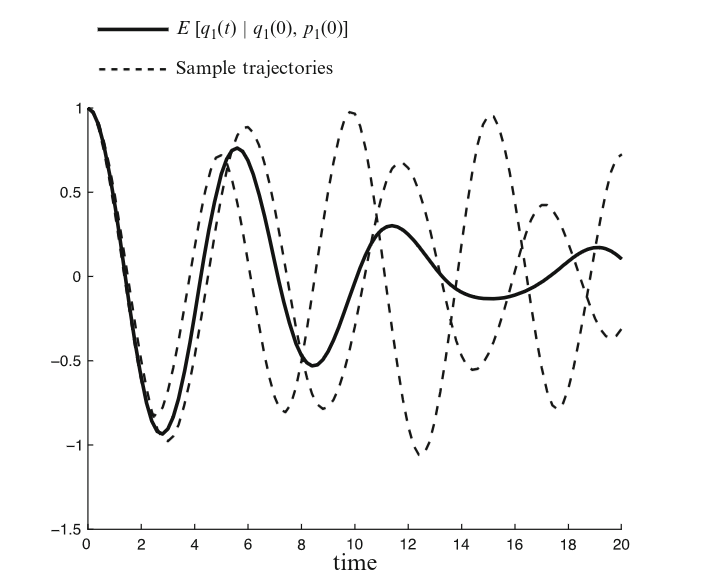
\includegraphics[width=0.4\textwidth]{03_SEMINARIO_MZ/02_APRESENTACAO/01_LATEX/img/grafico_motivacao.png}
		\caption{Simulação - Exemplo motivador}
		\label{fig:simulacao_exemplo_motivador}
	\end{figure}
\end{frame}

\section{Prolegômenos}

\begin{frame}{EDOs como EDPs lineares}
	
	A partir do sistema de EDO:
	\begin{equation*}
		\frac{d}{dt} \phi(x,t) = R(\phi(x,t)), \quad \phi(x,0) = x
	\end{equation*}
	
	Define-se o Operador de Liouville:
	\begin{equation*}
		L = \sum_i R_i(x) \frac{\partial}{\partial x_i}
	\end{equation*}
	
	Assim, temos o sistema equivalente de EDP:
	\begin{equation*}
		u_t = Lu, \quad u(x,0) = g(x), \quad u(x,t) = g(\phi(x,t))
	\end{equation*}
	
\end{frame}
%--------------------------------------------------------

\begin{frame}{Notação de semigrupo}
	\begin{itemize}
		\item Usada para representar soluções de EDPs de forma compacta.
		\item Exemplo: equação do calor
		      \begin{equation*}
		      	v_t - \frac{1}{2}\Delta v = 0, \quad v(x,0) = \phi(x)
		      \end{equation*}
		\item Solução escrita como:
		      \begin{equation*}
		      	v(t) = e^{\frac{1}{2}t\Delta} \phi
		      \end{equation*}
		\item Propriedade: $e^{(t+s)\Delta} = e^{t\Delta} e^{s\Delta}$
	\end{itemize}
\end{frame}

%--------------------------------------------------------

\begin{frame}{Aplicando ao Operador de Liouville}
	\begin{itemize}
		\item Solução da EDP:
		      \begin{equation*}
		      	e^{tL}g(x) = g(\phi(x,t))
		      \end{equation*}
		\item $g$ comuta com a evolução do sistema.
		\item Relação de comutação:
		      \begin{equation*}
		      	Le^{tL} = e^{tL}L
		      \end{equation*}
		\item Para matrizes: fórmula de Dyson:
		      \begin{equation*}
		      	\exp(t(A+B)) = \exp(tA) + \int_0^t \exp((t-s)(A+B)) B \exp(sA)\, ds
		      \end{equation*}
	\end{itemize}
\end{frame}

%--------------------------------------------------------

\begin{frame}{Produto interno hermitiano}
	\begin{itemize}
		\item Produto interno unidimensional:
		      \begin{equation*}
		      	\langle u, v \rangle = \int_{-\infty}^{+\infty} \frac{e^{-x^2/2}}{\sqrt{2\pi}} u(x)v(x)\, dx
		      \end{equation*}
		\item Ortogonalidade: $\langle p_n, p_m \rangle = 0$ se $n \neq m$
		\item Normalização: $\langle p_n, p_n \rangle = 1$
	\end{itemize}
\end{frame}

\begin{frame}{Extensão $n$-dimensional}
	\begin{itemize}
		\item Produto interno generalizado:
		      \begin{equation*}
		      	\langle u, v \rangle = \int \cdots \int (2\pi)^{-n/2} e^{-\sum \frac{x_i^2}{2}} u(x)v(x)\, dx
		      \end{equation*}
		\item Possibilidade de definir polinômios ortonormais em $q$, $p$ com densidade $e^{-H/T}$
	\end{itemize}
\end{frame}

%--------------------------------------------------------

\begin{frame}{Projeção e Mori-Zwanzig}
	\begin{itemize}
		\item Espaço $\Gamma$ $n$-dimensional com densidade de probabilidade.
		\item Divide-se $x$ em $\hat{x}$ (resolvidas) e $\tilde{x}$ (não resolvidas).
		\item Projeção ortogonal: $\mathbb{P}g = \mathbb{E}[g \mid \hat{x}]$
		\item Subespaço gerado por polinômios hermitianos em $\hat{x}$.
	\end{itemize}
\end{frame}
\section{Mori-Zwanzig}

\begin{frame}{Construção do formalismo MZ}
\begin{itemize}
    \item Separação das variáveis: $x = (\hat{x}, \tilde{x})$ e $\phi = (\hat{\phi}, \tilde{\phi})$ e $R = (\hat{R}, \tilde{R})$
    \item Foco nas $m$ primeiras componentes: variáveis resolvidas.
    \item Escrevemos: $\hat{\phi}_j(x,t) = e^{tL}x_j$, $1 \leq j \leq m$
    \item Derivando no tempo:
    \begin{equation*}
        \frac{\partial}{\partial t}e^{tL}x_j = e^{tL}Lx_j
    \end{equation*}
    \item Com projeções ortogonais: $\mathbb{Q} = I - \mathbb{P}$
\end{itemize}
\end{frame}

%--------------------------------------------------------

\begin{frame}{Equação de Mori-Zwanzig via Dyson}
\begin{itemize}
    \item Fórmula de Dyson aplicada:
    \begin{equation*}
        e^{tL} = e^{t\mathbb{Q}L} + \int_0^t e^{(t-s)L} \mathbb{P}L e^{s\mathbb{Q}L} \, ds
    \end{equation*}
    \item Substituindo na equação de evolução:
    \begin{equation*}
        \frac{\partial}{\partial t} e^{tL} x_j = \ e^{tL} \mathbb{P}L x_j + e^{t\mathbb{Q}L} \mathbb{Q}L x_j + \int_0^t e^{(t-s)L} \mathbb{P}L e^{s\mathbb{Q}L} \mathbb{Q}L x_j \, ds
    \end{equation*}
\end{itemize}
\end{frame}

%--------------------------------------------------------

\begin{frame}{Análise termo a termo}
    Vamos decompor o termo $e^{tL} x_j$ segundo a equação de Mori-Zwanzig, analisando separadamente:
    \begin{itemize}
        \item O termo markoviano (primeiro termo),
        \item O termo de ruído (segundo termo),
        \item O termo de memória (terceiro termo).
    \end{itemize}
\end{frame}

%--------------------------------------------------------

\begin{frame}{Primeiro termo}
O primeiro termo é dado por:
\begin{equation}
	e^{tL} \mathbb{P}L x_j
	\label{eq:primeiro-termo-mz}
\end{equation}

A partir dele, temos que:
\begin{align*}
	Lx_j &= \sum_i R_i\left(\frac{\partial}{\partial x_i}\right)x_j = R_j(x), \\
	\mathbb{P}Lx_j &= \mathbb{E}[R_j(x)\,|\,\hat{x}], \\
	e^{tL}\mathbb{P}Lx_j &= \bar{R}_j\left(\hat{\phi}(x,t)\right).
\end{align*}

\footnotesize{Note que é um termo markoviano, pois depende apenas do estado atual $\hat{\phi}(x,t)$.}
\end{frame}

%--------------------------------------------------------

\begin{frame}{Segundo termo}

O segundo termo é dado por:
\begin{equation*}
	w_j = e^{t\mathbb{Q}L} \mathbb{Q}L x_j
\end{equation*}

A partir dele, temos que:
\begin{align}
	\frac{\partial}{\partial t} w_j(x,t) &= \mathbb{Q}L w_j(x,t), \nonumber\\
	w_j(x,0) &= \mathbb{Q}L x_j = R_j(x) - \mathbb{E}[R_j \mid \hat{x}]. 
    \label{eq:mori-zwanzig-dinamica-ortogonal}
\end{align}

A função $w_j(x,0)$ representa a \textit{parte flutuante} de $R_j(x)$ e evolui segundo a dinâmica ortogonal. Temos $\mathbb{P} w_j(x,t) = 0$ para todo $t$.
\end{frame}

%--------------------------------------------------------

\begin{frame}{Subespaço de ruído}
O \textit{subespaço do ruído} é formado por funções ortogonais às funções de $\hat{x}$.

Isso corresponde, geralmente, a termos que dependem de $\tilde{x}$. Esses termos são imprevisíveis dado $\hat{x}$.
\end{frame}

\begin{frame}{Terceiro termo}

O terceiro termo é dado por:
\begin{equation*}
	\int_0^t e^{(t-s)L} \mathbb{P}L e^{s\mathbb{Q}L} \mathbb{Q}L x_j
\end{equation*}
Este termo depende do histórico do sistema: é o \textbf{termo de memória}.

Projeção usando polinômios hermitiano $H_1, H_2, \dots$:
\begin{align*}
	\mathbb{P}L e^{s\mathbb{Q}L} \mathbb{Q}L x_j &= \sum_k \langle L\mathbb{Q} e^{s\mathbb{Q}L} \mathbb{Q}Lx_j, H_k(\hat{x}) \rangle H_k(\hat{x}).
\end{align*}
\end{frame}

%--------------------------------------------------------

\begin{frame}{Produto interno e antissimetria de $L$}
Se $L$ é antissimétrico: $(u, Lv) = -(Lu, v)$, então:
\begin{align*}
	(L \mathbb{Q} e^{s \mathbb{Q} L} \mathbb{Q}L x_j, H_k) 
	  &= - (\mathbb{Q} e^{s \mathbb{Q} L} \mathbb{Q}L x_j, L H_k) \\
	  &= - (e^{s \mathbb{Q} L} \mathbb{Q}L x_j, \mathbb{Q}L H_k).
\end{align*}

O terceiro termo é uma soma de covariâncias temporais de ruído.
\end{frame}

\section{De volta ao sistema motivador}

%--------------------------------------------------------
\begin{frame}{Sistema hamiltoniano}
	Vamos relembrar o sistema trabalhado:
	\begin{equation*}
		H = \frac{1}{2}(q_1^2 + q_2^2 + q_1^2 q_2^2 + p_1^2 + p_2^2)
	\end{equation*}
	\begin{align*}
		\dot{q}_1 & = p_1, & \dot{p}_1 & = -q_1(1 + q_2^2), \\
		\dot{q}_2 & = p_2, & \dot{p}_2 & = -q_2(1 + q_1^2)  
	\end{align*}
\end{frame}

%--------------------------------------------------------
\begin{frame}{Operador e densidade}
	A evolução temporal é governada pelo operador de Liouville:
    \begin{equation*}
        L = p_1 \frac{\partial}{\partial q_1} - q_1(1 + q_2^2)\frac{\partial}{\partial p_1} + p_2 \frac{\partial}{\partial q_2} - q_2(1 + q_1^2)\frac{\partial}{\partial p_2}.
    \end{equation*}

	As variáveis não resolvidas seguem uma distribuição canônica com temperatura $T=1$:
	\begin{equation*}
		W(x) = \exp\left(\frac{-H(q,p)}{Z}\right)
	\end{equation*}
\end{frame}

%--------------------------------------------------------
\begin{frame}{Primeira aproximação: Modelo-$t$}
	Para simplificar o termo de memória, usamos a chamada aproximação modelo-$t$:
	\begin{equation*}
		\int_0^t e^{(t-s)L} \mathbb{P}L e^{s \mathbb{Q}L} ds \approx t e^{tL} \mathbb{P}L \mathbb{Q}L x_j
	\end{equation*}
	Chegamos à seguinte equação aproximada:
	\begin{equation*}
		\frac{d}{dt} e^{tL} \hat{x} = e^{tL} \mathbb{P}L \hat{x} + t e^{tL} \mathbb{P}L \mathbb{Q}L \hat{x} + e^{tL} \mathbb{Q}L \mathbb{Q}L x_j
	\end{equation*}
\end{frame}

%--------------------------------------------------------
\begin{frame}{Sistema com ruído}
	Com isso, as equações para $q_1$ e $p_1$ se tornam:
	\begin{align*}
		\frac{d}{dt} q_1 & = p_1,                                                                                                              \\
		\frac{d}{dt} p_1 & = -q_1\left(1 + \frac{1}{1 + q_1^2}\right) - 2t\frac{q_1^2 p_1}{(1 + q_1^2)^2} + e^{tL} \mathbb{Q}L \mathbb{Q}L p_1 
	\end{align*}
	O termo final representa o ruído originado pelas variáveis não resolvidas.
\end{frame}

%--------------------------------------------------------
\begin{frame}{Esperanças condicionais}
	Nosso objetivo é estimar:
	\begin{equation*}
		\mathbb{E}[q_1(t) | q_1(0), p_1(0)], \quad \mathbb{E}[p_1(t) | q_1(0), p_1(0)]
	\end{equation*}
	Ao aplicar o operador $\mathbb{P}$ às equações anteriores, o termo de ruído desaparece.
\end{frame}

%--------------------------------------------------------
\begin{frame}{Segunda aproximação}
	Adotamos uma segunda aproximação: comutação entre média e função.
	\begin{equation*}
		\mathbb{E}[(1 + q_1^2(t))^{-1} | q_1(0), p_1(0)] \approx \left(1 + \mathbb{E}[q_1(t)]^2\right)^{-1}
	\end{equation*}
	Com isso, definimos:
	\begin{equation*}
		Q_1(t) = \mathbb{E}[q_1(t)], \quad P_1(t) = \mathbb{E}[p_1(t)]
	\end{equation*}
\end{frame}

%--------------------------------------------------------
\begin{frame}{Sistema final}
	Finalmente, obtemos o sistema determinístico aproximado:
	\begin{align*}
		\frac{d}{dt} Q_1 & = P_1,                                                                                  \\
		\frac{d}{dt} P_1 & = -Q_1\left(1 + \frac{1}{1 + Q_1^2} \right) - t \cdot \frac{2 Q_1^2 P_1}{(1 + Q_1^2)^2} 
	\end{align*}
	Essa é a versão suavizada das equações iniciais, onde os efeitos do ruído foram absorvidos pela média.
\end{frame}

%--------------------------------------------------------

\begin{frame}{Gráfico}
	\begin{figure}[h]
		\centering
		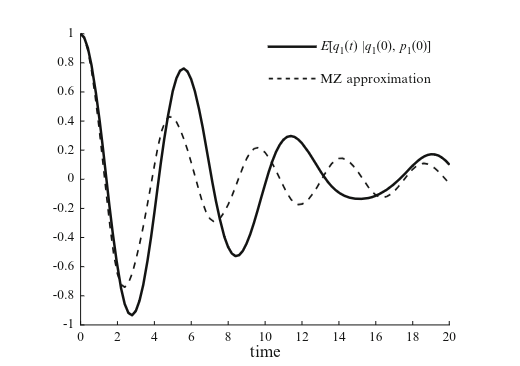
\includegraphics[width=0.4\textwidth]{03_SEMINARIO_MZ/02_APRESENTACAO/01_LATEX/img/grafico_motivacao_mz.png}
		\caption{Simulação - Exemplo motivador com o método Mori-Zwanzig}
		\label{fig:simulacao_exemplo_motivador_mz}
	\end{figure}
\end{frame}


\section{Conclusão} % Seções são adicionadas para organizar sua apresentação em blocos discretos, todas as seções e subseções são automaticamente exibidas no índice como uma visão geral da apresentação, mas NÃO são exibidas como slides separados.

\begin{frame}{Principais dúvidas}
    \begin{enumerate}
        \item Equação densidade probabilidade canônica;
        \item Valor esperado de funções
        \item Hamiltonianos, sistemas hamiltonianos
        \item Espaço de projeção
        \item Segunda aproximação
    \end{enumerate}
\end{frame}
\begin{frame}{Referências}
    \nocite{*}
    \printbibliography[heading=none]
\end{frame}

% Slide final
\begin{frame}
    \begin{center}
        {\Huge Fim da apresentação!}
    \end{center}
\end{frame}

\end{document}